\section{Theorie} 
\label{sec:Theorie}

In diesem Kapitel werden die theoretischen Hintergründe dieses Versuches erläutert. Dabei wird insbesondere auf die in der Durchführung verwendeten Schaltungen eingegangen.

\begin{figure}
    \centering
    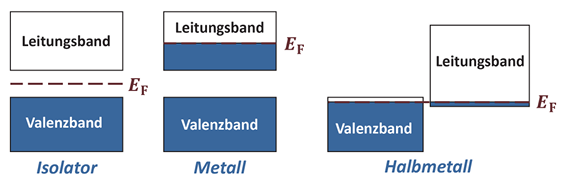
\includegraphics[width=1\textwidth]{content/grafiken/baender.JPG}
    \caption{Vergleich der Bändermodelle von Isolatoren, Leitern und Halbleitern. $E_F$ bezeichnet die Fermienergie [1]}
    \label{fig:baendermodell}
  \end{figure}

  \begin{figure}
    \centering
    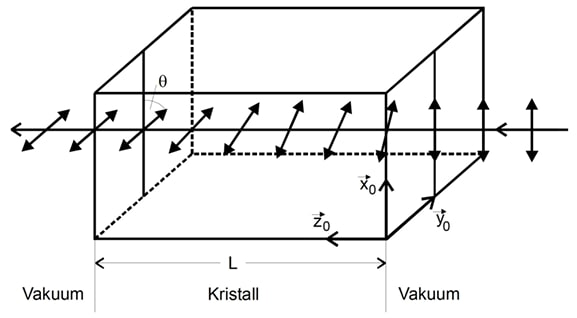
\includegraphics[width=1\textwidth]{content/grafiken/kristall.JPG}
    \caption{Drehung der Polarisationsebene einer elekromagnetischen Welle im B-Feld durchfluteten Medium. [1]}
    \label{fig:kristall}
  \end{figure}